\chapter{Méthode + Théorie}

\section{Structure d'une protéine et d'un complexe}

L'objectif du projet étant de modéliser l'interface de contact entre deux protéines,
il est important de comprendre la structure d'une protéine. Nous verrons également
comment sont stockées ces structures, grâce au fichiers \textit{.pdb}.

\subsection{Structure}

Les protéines sont des molécules biologiques présentes dans toutes les cellules vivantes.
Elles sont constituées d'un enchaînement d'acides aminés.
Les protéines assurent diverses fonctions au sein de la cellule vivante et dans les tissus.
Elles peuvent avoir un rôle enzymatique, structurel, permettre la mobilité des molécules, la
régulation de l'expression génétique ou encore transmettre des signaux cellulaires.
Les chaînes protéiques constituant les protéines sont synthétisées dans la cellule. Le
matériel génétique de la cellule détermine l'ordre d'enchainement des acides aminés.
Les protéines adoptent alors une structure en trois dimensions qui leur permet d'assurer
 leur fonction biologique. Les protéines peuvent interagir ensemble afin d'assurer certaines
fonctions biologiques. Ces interactions forment des complexes protéiques. Les structures
 des protéines et leurs interactions sont particulièrement utilisées en chimie médicinale.
L'étude des surfaces et des espaces disponibles peut guider la recherche d'un nouveau
médicament. La cristallographie est utilisée pour étudier la structure des protéines à
l'échelle atomique. Elle s'appuie sur le phénomène physique de diffraction des ondes
électromagnétiques (rayons X).

\subsection{Fichier de stockage}

Les données utilisables d'une protéine (ou d'un complexe) sont stockées grâce aux
fichiers \textit{.pdb}. Ces fichiers, leur lecture et l'interprétation des données
qu'ils contiennent, sont essentiels à l'observation des protéines. En effet, chaque
ligne, exceptée la première, correspond à un atome composant la protéine étudiée.
Ces lignes contiennent des informations telles que la chaîne à laquelle appartient
l'atome, son acide aminé ou ses coordonnées dans l'espace (en $\si{\angstrom}$).

\begin{figure}[ht]
  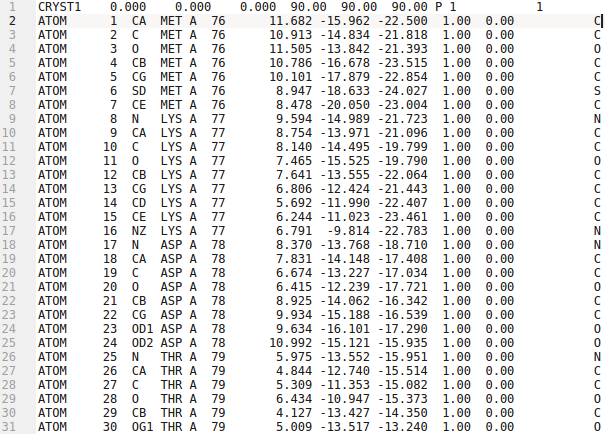
\includegraphics[width=\textwidth]{figures/pdb_example.png}
  \caption{Exemple de fichier .pdb}
  \label{fig::pdb_file}
\end{figure}



\section{Triangulation de Delaunay}

Une protéine est donc représentée comme un nuage de points où chacun de ces points
représente un atome de la protéine. Dans le but d'optimiser les temps de parcours dans
ce nuage de points et de modéliser l'interface entre les deux protéines,
 on utilise la triangulation de Delaunay.

 Cette triangulation est unique et peut être expliquée de la manière suivante :
 chaque cercle circonscrit à un triangle du nuage de point ne contient que les points
 dudit triangle (voir figure \ref{fig::explication_delaunay}). Nous expliquerons dans un premier
 temps la méthode pour déterminer l'interface en deux dimensions.

\begin{figure}[ht]
\centering
  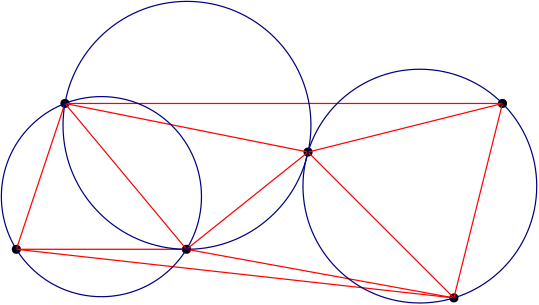
\includegraphics[width=\textwidth]{figures/explication_delaunay.png}
  \caption{Triangulation de Delaunay}
  \label{fig::explication_delaunay}
\end{figure}

\subsection{Dimension 2}

Il faut appliquer cette triangulation au complexe dont on veut déterminer l'interface, c'est-à dire
aux points donnés par les coordonnées des atomes qui composent le complexe
(voir figure \ref{fig::delaunay_tr}). Les protéines du complexe sont différenciées
par leurs couleurs (rouge et bleu) sur le schéma. Nous sélectionnons alors la partie utile de
cette triangulation (voir figure \ref{fig::delaunay_reduced}) : nous ne gardons que
les triangles qui contiennent au moins un point à l'interface.
Un point est à l'interface s'il appartient à un triangle contenant au moins un point
de chaque protéine. Le fait de réduire la taille de la triangulation sera utile par la suite
pour accélérer les temps de traitement et de récupération de données concernant l'interface.



\begin{figure}[ht]
\centering
\begin{subfigure}{0.4\textwidth}
  \centering
  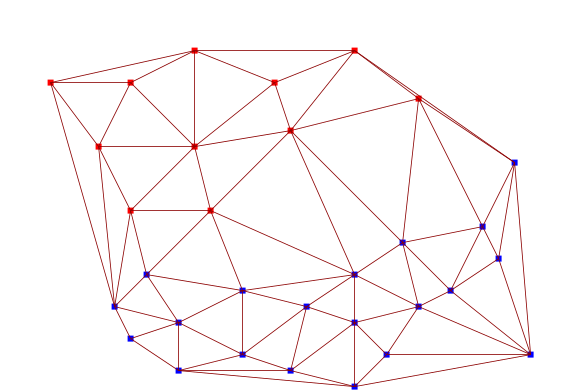
\includegraphics[width=\textwidth]{figures/delaunay.png}
  \caption{Triangulation de Delaunay}
  \label{fig::delaunay_tr}
\end{subfigure}%
\begin{subfigure}{0.2\textwidth}
  \centering
  $\Longrightarrow$
\end{subfigure}%
\begin{subfigure}{0.4\textwidth}
  \centering
  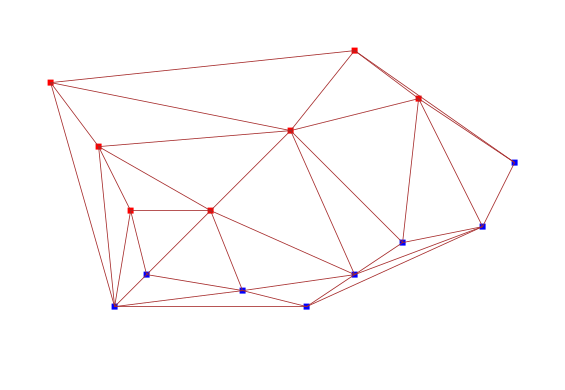
\includegraphics[width=\textwidth]{figures/delaunay_reduced.png}
  \caption{Triangulation réduite}
  \label{fig::delaunay_reduced}
\end{subfigure}
\caption{Réduction d'une triangulation}
\label{fig::delaunays}
\end{figure}

Nous nous intéressons maintenant à la détermination de l'interface, proprement dite.
En ne gardant que les arêtes utiles (voir figure \ref{fig::delaunays_process_1}),
c'est-à-dire celles reliant deux points appartenant
à deux protéines différentes, nous pouvons approximer l'interface de contact grâce
au diagramme de Voronoï.

\begin{figure}[ht]
\centering
\begin{subfigure}{0.45\textwidth}
  \centering
  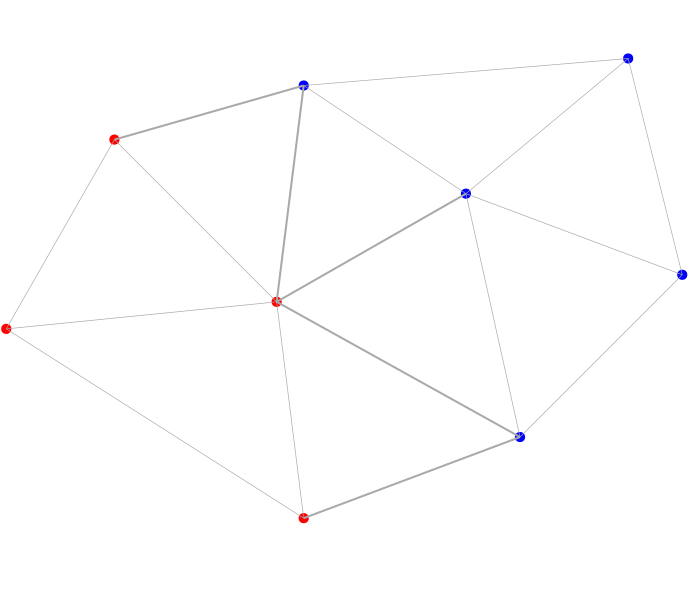
\includegraphics[width=\textwidth]{figures/process_d_1.png}
  \caption{Triangulation de Delaunay}
  \label{fig::process_d_1}
\end{subfigure}%
\begin{subfigure}{0.1\textwidth}
  \centering
  $\Longrightarrow$
\end{subfigure}%
\begin{subfigure}{0.45\textwidth}
  \centering
  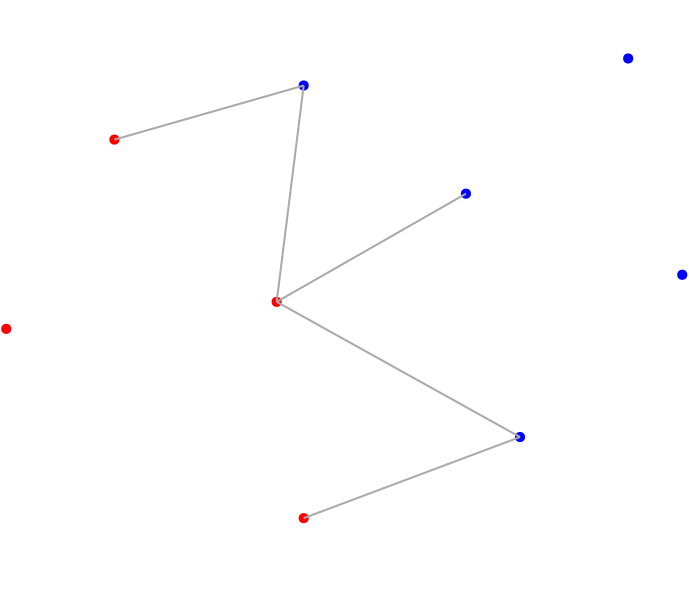
\includegraphics[width=\textwidth]{figures/process_d_2.png}
  \caption{Arêtes à l'interface}
  \label{fig::process_d_2}
\end{subfigure}
\caption{Triangulations et zone utile}
\label{fig::delaunays_process_1}
\end{figure}


Ce diagramme est le dual de la triangulation de Delaunay et représente les points à
égale distance des points de la triangulation (voir figure \ref{fig::process_d_3}).
En ne gardant que les parties du giagramme de Voronoï qui correspondent au arêtes sélectionnées
précédemment (voir figure \ref{fig::process_d_4}), nous obtenons une doite par morceau
qui approxime l'interface de contact en dimension 2.

\begin{figure}[ht]
\centering
\begin{subfigure}{0.45\textwidth}
  \centering
  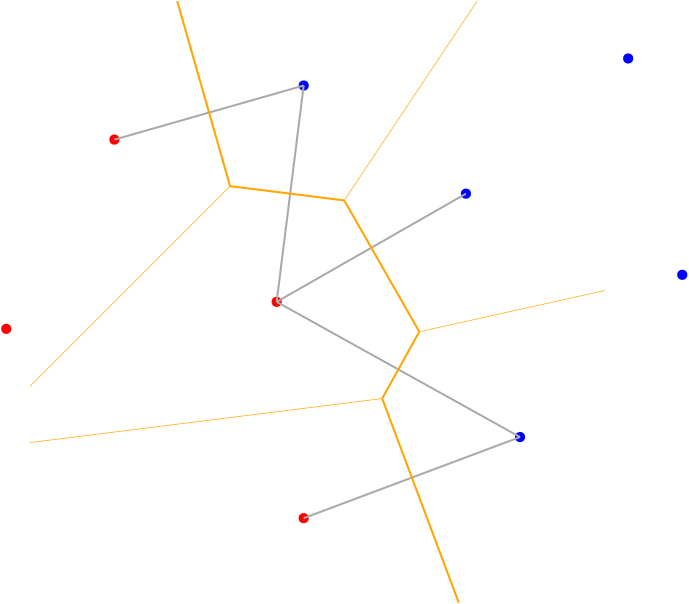
\includegraphics[width=\textwidth]{figures/process_d_3.png}
  \caption{Diagramme de Voronoï}
  \label{fig::process_d_3}
\end{subfigure}%
\begin{subfigure}{0.1\textwidth}
  \centering
  $\Longrightarrow$
\end{subfigure}%
\begin{subfigure}{0.45\textwidth}
  \centering
  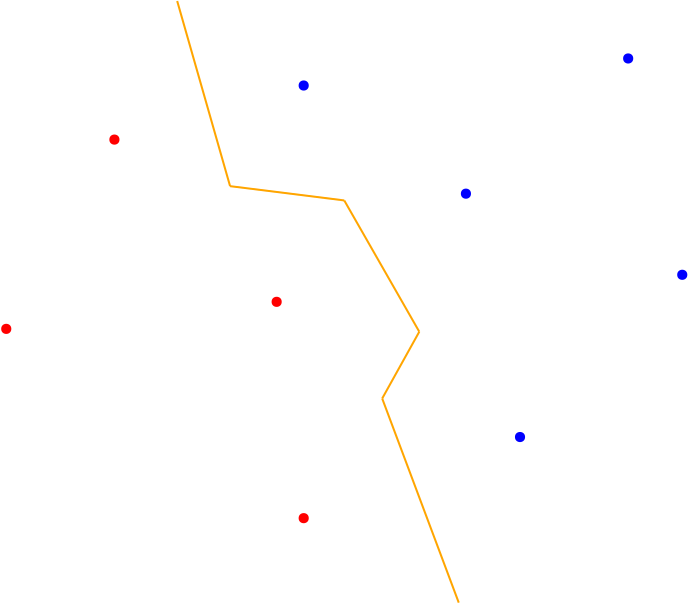
\includegraphics[width=\textwidth]{figures/process_d_4.png}
  \caption{Interface}
  \label{fig::process_d_4}
\end{subfigure}
\caption{Recherche de la surface de contact}
\label{fig::delaunays_process_2}
\end{figure}


\subsection{Dimension 3}

Si nous transposons la méthode vue ci-dessus en dimension 3, les triangles formés
par les points deviennent des tetrahèdres sur lesquels nous travaillerons pour vérifier
les zones utiles au calcul de l'interface.
De plus, le dual d'une arêtes devient une surface entourant cette arête. En rassemblant ces morceaux
de surface, nous obtenons une surface en trois dimension qui modélise la surface
de contact entre les deux protéines du complexe étudié.

\begin{figure}[ht]
\centering
\begin{subfigure}{0.45\textwidth}
  \centering
  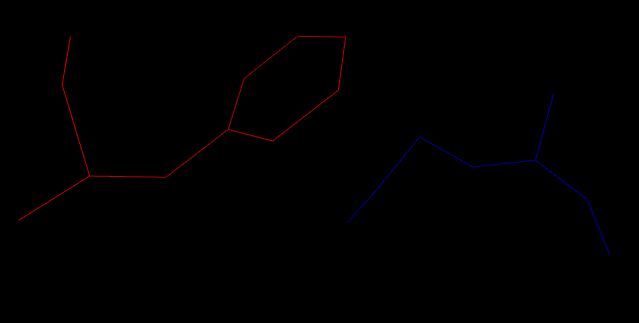
\includegraphics[width=\textwidth]{figures/small_prot.png}
  \caption{Partie d'un complexe}
  \label{fig::small_prot}
\end{subfigure}%
\begin{subfigure}{0.1\textwidth}
  \centering
  $\Longrightarrow$
\end{subfigure}%
\begin{subfigure}{0.45\textwidth}
  \centering
  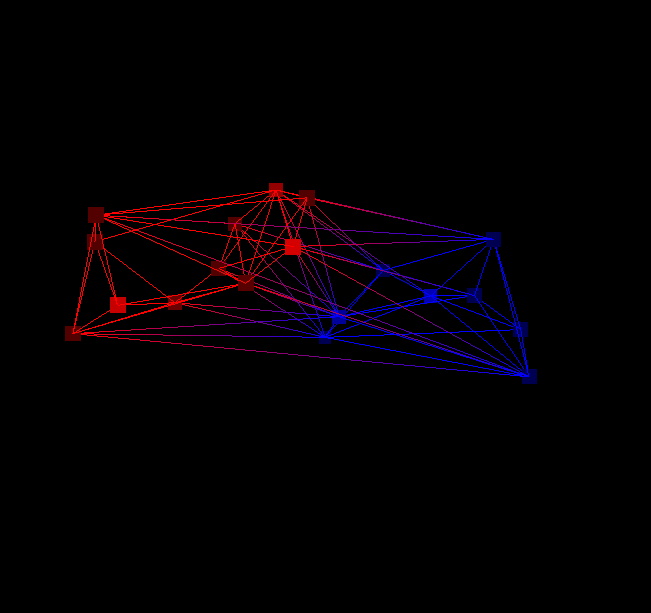
\includegraphics[width=\textwidth]{figures/3d_triangulation04.png}
  \caption{Triangulation}
  \label{fig::prot_delaunay}
\end{subfigure}
\caption{Triangulation 3D d'un complexe}
\label{fig::delaunays_3d}
\end{figure}

\section{CGAL}
\begin{itemize}
  \item Structures
  \item Iterateurs
  \item Compilation -> Cmake
\end{itemize}

Pour développer la méthode vue précédemment, nous avons choisi d'utiliser CGAL
(Computational Geometry Algorithms Library).
CGAL est un projet logiciel qui fournit un accès libre à de nombreux algorithmes géométriques
efficaces et fiables sous forme d'une bibliothèque C++. CGAL est utilisé dans des
domaines diverses ayant besoin de calcul géométrique, tels que des systèmes
d'information géographiques, la conception assistée par ordinateur, la biologie
moléculaire, l'imagerie médicale, l'infographie et la robotique.

Nous nous sommes particulièrement intéressés à une partie de CGAL qui permet le
stockage de nuages de points sous forme de triangulations de Delaunay. L'avantage
de cette bibliothèque réside dans les structure et les méthodes accélérant les différentes
étapes du calcul de l'interface entre deux protéines.

\subsection{Structures}


En effet, CGAL comprend notamment une structure \textit{Delaunay\_Triangulation\_3},
permettant de calculer et de stocker une triangulation de Delaunay depuis de simples
tableaux (\textit{C++ Arrays}) listant des points dans l'espace. Pour mieux, comprendre
l'implémentation réalisée durant ce projet, il est important de préciser la structure des tétrahèdres
composant une trianguation de Delaunay (voir figure \ref{fig::tetrahedron_cgal}).

\begin{figure}[ht]
\centering
  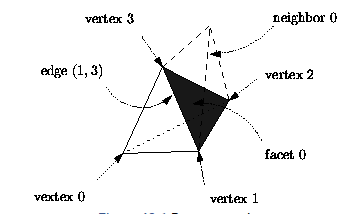
\includegraphics[width=0.5\textwidth]{figures/tetrahedron_cgal.png}
  \caption{Structure d'un tetrahèdre dans CGAL}
  \label{fig::tetrahedron_cgal}
\end{figure}

Un tetrahèdre est représenté par quatre entités :
\begin{itemize}
  \item Vertex : contient un point (coordonnées 3D)
  \item Edge : une arête contenant deux vertex ordonnés et une cellule
  \item Facet : une face stockée grâce à une cellule et le vertex qui lui est opposé dans cette cellule
  \item Cell : un tetrahèdre qui donne accès à quatre vertex et quatre cellules adjacentes
\end{itemize}









\subsection{Itérateurs}

Les itérateurs sont une généralisation de pointeur qui permettent de travailler sur
différentes structures de données.
Il existe des itérateurs permettant de parcourir une triangulation de Delaunay
selon chacune des entités formant celle-ci : vertice, arête, face, cellule. Quelle
que soit l'entité utilisée, il est possible d'accéder au trois autres entités et
aux données qu'elle contiennent.

\subsection{Compilation}
